\documentclass[a4paper]{report}
\usepackage{amsmath}
\usepackage{ulem}
\usepackage{ngerman}
\usepackage{graphicx}
\usepackage{subfig}
\usepackage[svgnames]{xcolor} % Required for colour specification
\newcommand*{\plogo}{\fbox{$\mathcal{PL}$}} % Generic dummy publisher logo
\renewcommand{\baselinestretch}{1.25}
\usepackage[T1]{fontenc} % Output font encoding for international characters
\usepackage[utf8]{inputenc} % Required for inputting international characters
\usepackage{tgadventor} % Use the Paratype Serif font
\renewcommand{\familydefault}{\sfdefault}
\usepackage{float}
\usepackage[hidelinks]{hyperref}
\usepackage{refstyle}
\usepackage{caption}
\usepackage{pdfpages}%
\usepackage{geometry}
 \geometry{
 left=30mm,
 top=30mm,
 bottom=20mm,
 }

\usepackage{fancyhdr}
\pagestyle{fancy}
\fancyhf{}
\rhead{MBE}
%\lhead{\LaTeX{} tutorials}
\lhead{\nouppercase{\rightmark} (\nouppercase{\leftmark})}
\rfoot{Page \thepage}
\renewcommand{\headrulewidth}{2pt}

	%------------------------------------------------
	%	Start der Beschreibung
	%------------------------------------------------
\begin{document}


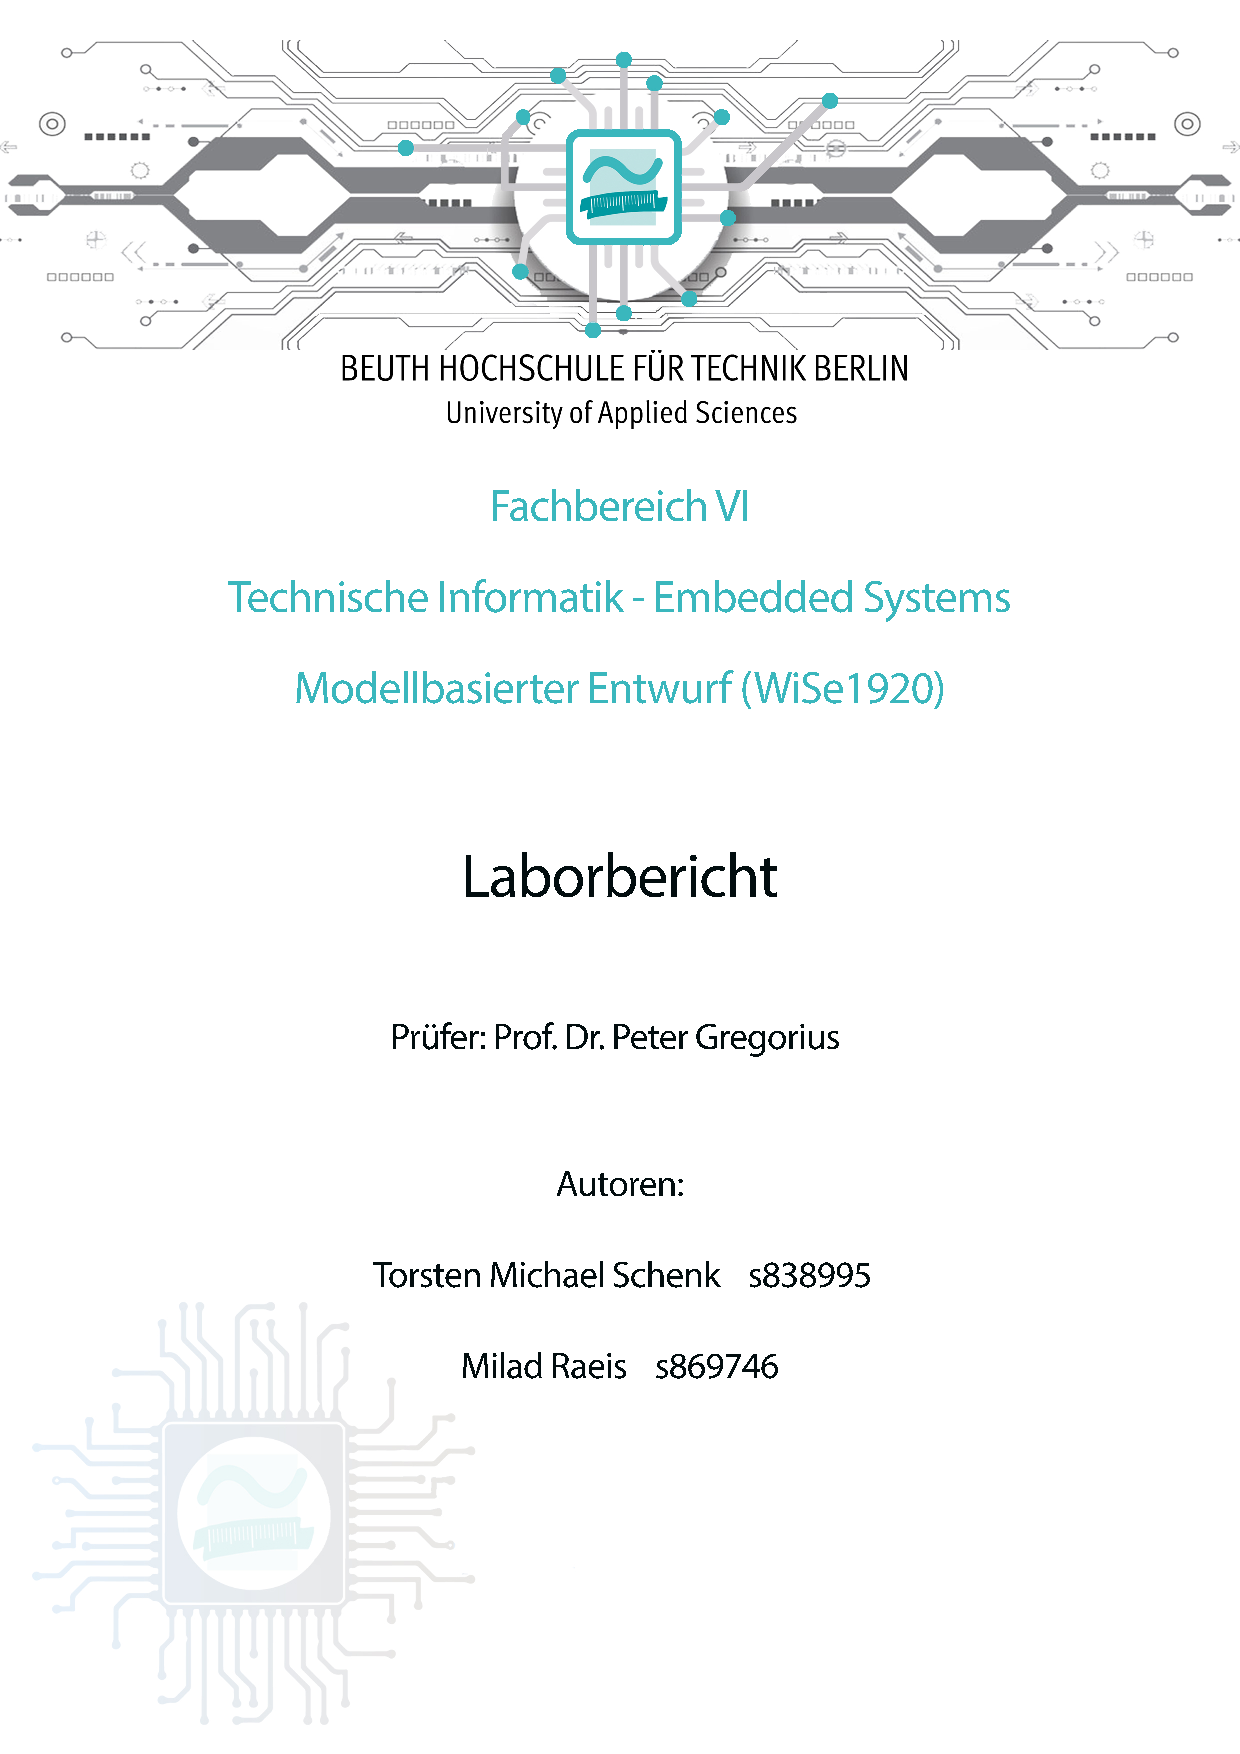
\includepdf{Coverpage.pdf}
\tableofcontents
\listoffigures




\section{Vorwort}
Bei der Recherche zur Bearbeitung der Übungen wurden viele englischsprachige Webseiten zu rate gezogen. Generell kann man sagen, dass englische Fachbegriffe sich im Bereich FPGA und embedded Design etabliert haben, so dass eine Übersetzung eher verwirren als helfen würde. Daher haben wir uns entschieden, die \textbf{englischen} Bezeichner und Beschreibungen beizubehalten.\\
Um Codeabschnitte besser von Beschreibungen besser unterscheiden zu können, wurde eine eigene Schriftart verwendet:
\begin{verbatim}
  Kommandozeilen Eingaben und Codesnippets werden wie HIER dargestellt.
\end{verbatim}

\chapter{Projektbeschreibung}
In diesem Projekt sollen die Momente von Regionen (Blobs) berechnet werden. Momente sind im englischen Sprachgebrauch etabliert und werden im Deutschen als Massenträgheitsmomente oder einfach Trägheitsmomente bezeichnet. Sie kommen zum Einsatz wo statische Kennwerte die Konturabhängig sind benötigt werden. Eine wichtige Fragestellung ist z.B. in welcher Richtung sich ein L-Profil biegen wird. Die kontinuierliche Darstellung von Momenten als Integral in dem I(x,y) die gesamte Fläche eines Querschnittes darstellt: $$M = \int \int I(i,j) dxdy$$

Diskret (Bildpixel) können durch Iteration über alle Pixel einer Region die Momente berechnet werden. Die allgemeine Formel kann für alle Kombinationen verwendet werden, z.B. $M_{00}$, $M_{01}$, $M_{20}$. Die Zahlen dienen hierbei gleichzeitig als Exponent p oder q.: $$M_{p,q} = \sum \sum i^p jp^q I(i,j)$$

	\begin{figure}[H]
	\centering
	\subfloat{
\includegraphics[width=9cm,height=6cm]{PIC/cbwimg}}
	\caption{Beispiel: binarisiertes Bild}
	\label{Entwurf des Projects}
	\end{figure}

Im Projekt soll auf Bildern jeweils mindestens eine Region selektiert werden. In diese soll zur Anzeige des Ergebnisses der Schwerpunkt und die Orientierung in Richtung der Achse mit höherem Biegemoment. In der folgenden Abbildung sind die Schwerpunkte lila und die Orientierung grün eingezeichnet.
	
	\begin{figure}[H]
	\centering
	\subfloat{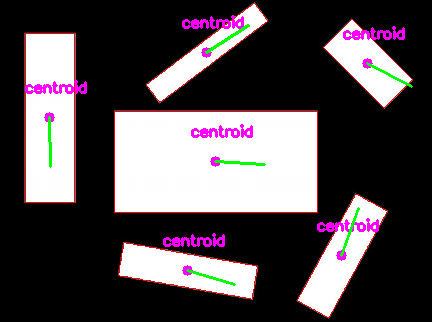
\includegraphics[width=9cm,height=6cm]{PIC/colorres}}
	\caption{Beispiel: Blobs mit Schwerpunkt und Richtung}
	\label{Entwurf des Projects}
	\end{figure}
	
Nach der binarisierung der Region können die Pixel jeder Region gezählt werden und sind in x und y Koordinaten im Bild bekannt. Zuerst werden die Schwerpunkte $\overline{x}$ und $\overline{y}$ berechnet. Danach erfolgt die Berechnung der Orientierung aus den Flächenmomenten mittels der Kovarianzen und der Kovarianzmatrix. \\

Schwerpunkt x: $$\overline{x} = \frac{M_{10}}{M_{00}}$$

Schwerpunkt y: $$\overline{y} = \frac{M_{01}}{M_{00}}$$

Kovarianzen: $$\mu_{20} = \frac{M_{20}}{M_{00}} - \overline{x}^2 $$
			 $$\mu_{11} = \frac{M_{11}}{M_{00}} - \overline{x}\overline{y} $$
			 $$\mu_{02} = \frac{M_{02}}{M_{00}} - \overline{y}^2 $$

     		$$cov(Obj) =\begin{bmatrix}
			 			\mu_{20} & \mu_{11}\\ 
				 		\mu_{11}& \mu_{02}
					 	\end{bmatrix}$$
			
			 
Orientierung einer Region im Wertebereich (+$\pi$, -$\pi$): $$ \theta = \frac{1}{2} tan^{-1}(\frac{2\mu_{11}}{\mu_{20}-\mu_{02}})    $$

Bei der Hardware Realisierung sind mehrere Optionen denkbar. Es werden FPGA Implementation für Kamera via PMOD und VGA über SHIELD PINs angestrebt. Sollte sich der mathematische Teil als \textbf{semesterfüllend} herausstellen, kann auf USB Kamera und HDMI Display (Anbindung über Pynq-Linux) ausgewichen werden. Im Worse-Case wäre noch das Laden und Speichern von Bildern aus einem Bildordner als Möglichkeit offen. \textbf{Im Vordergrund steht die Implementation der mathematischen Funktionen deren Verarbeitung im FPGA erfolgt.}

	%------------------------------------------------
	%	1. Chapter
	%------------------------------------------------

\chapter{Hardware}

In diesem Kapitel wird die für das Projekt erforderliche Hardware dargestellt und erläutert. Optional kann im Projekt die Kamera auf zwei verschiedene Arten angeschlossen werden. Die erste Möglichkeit ist über Verwendung des HDMI-Ports einen Bilschirm anzuschließen:
	\begin{figure}[H]
	\centering
	\subfloat{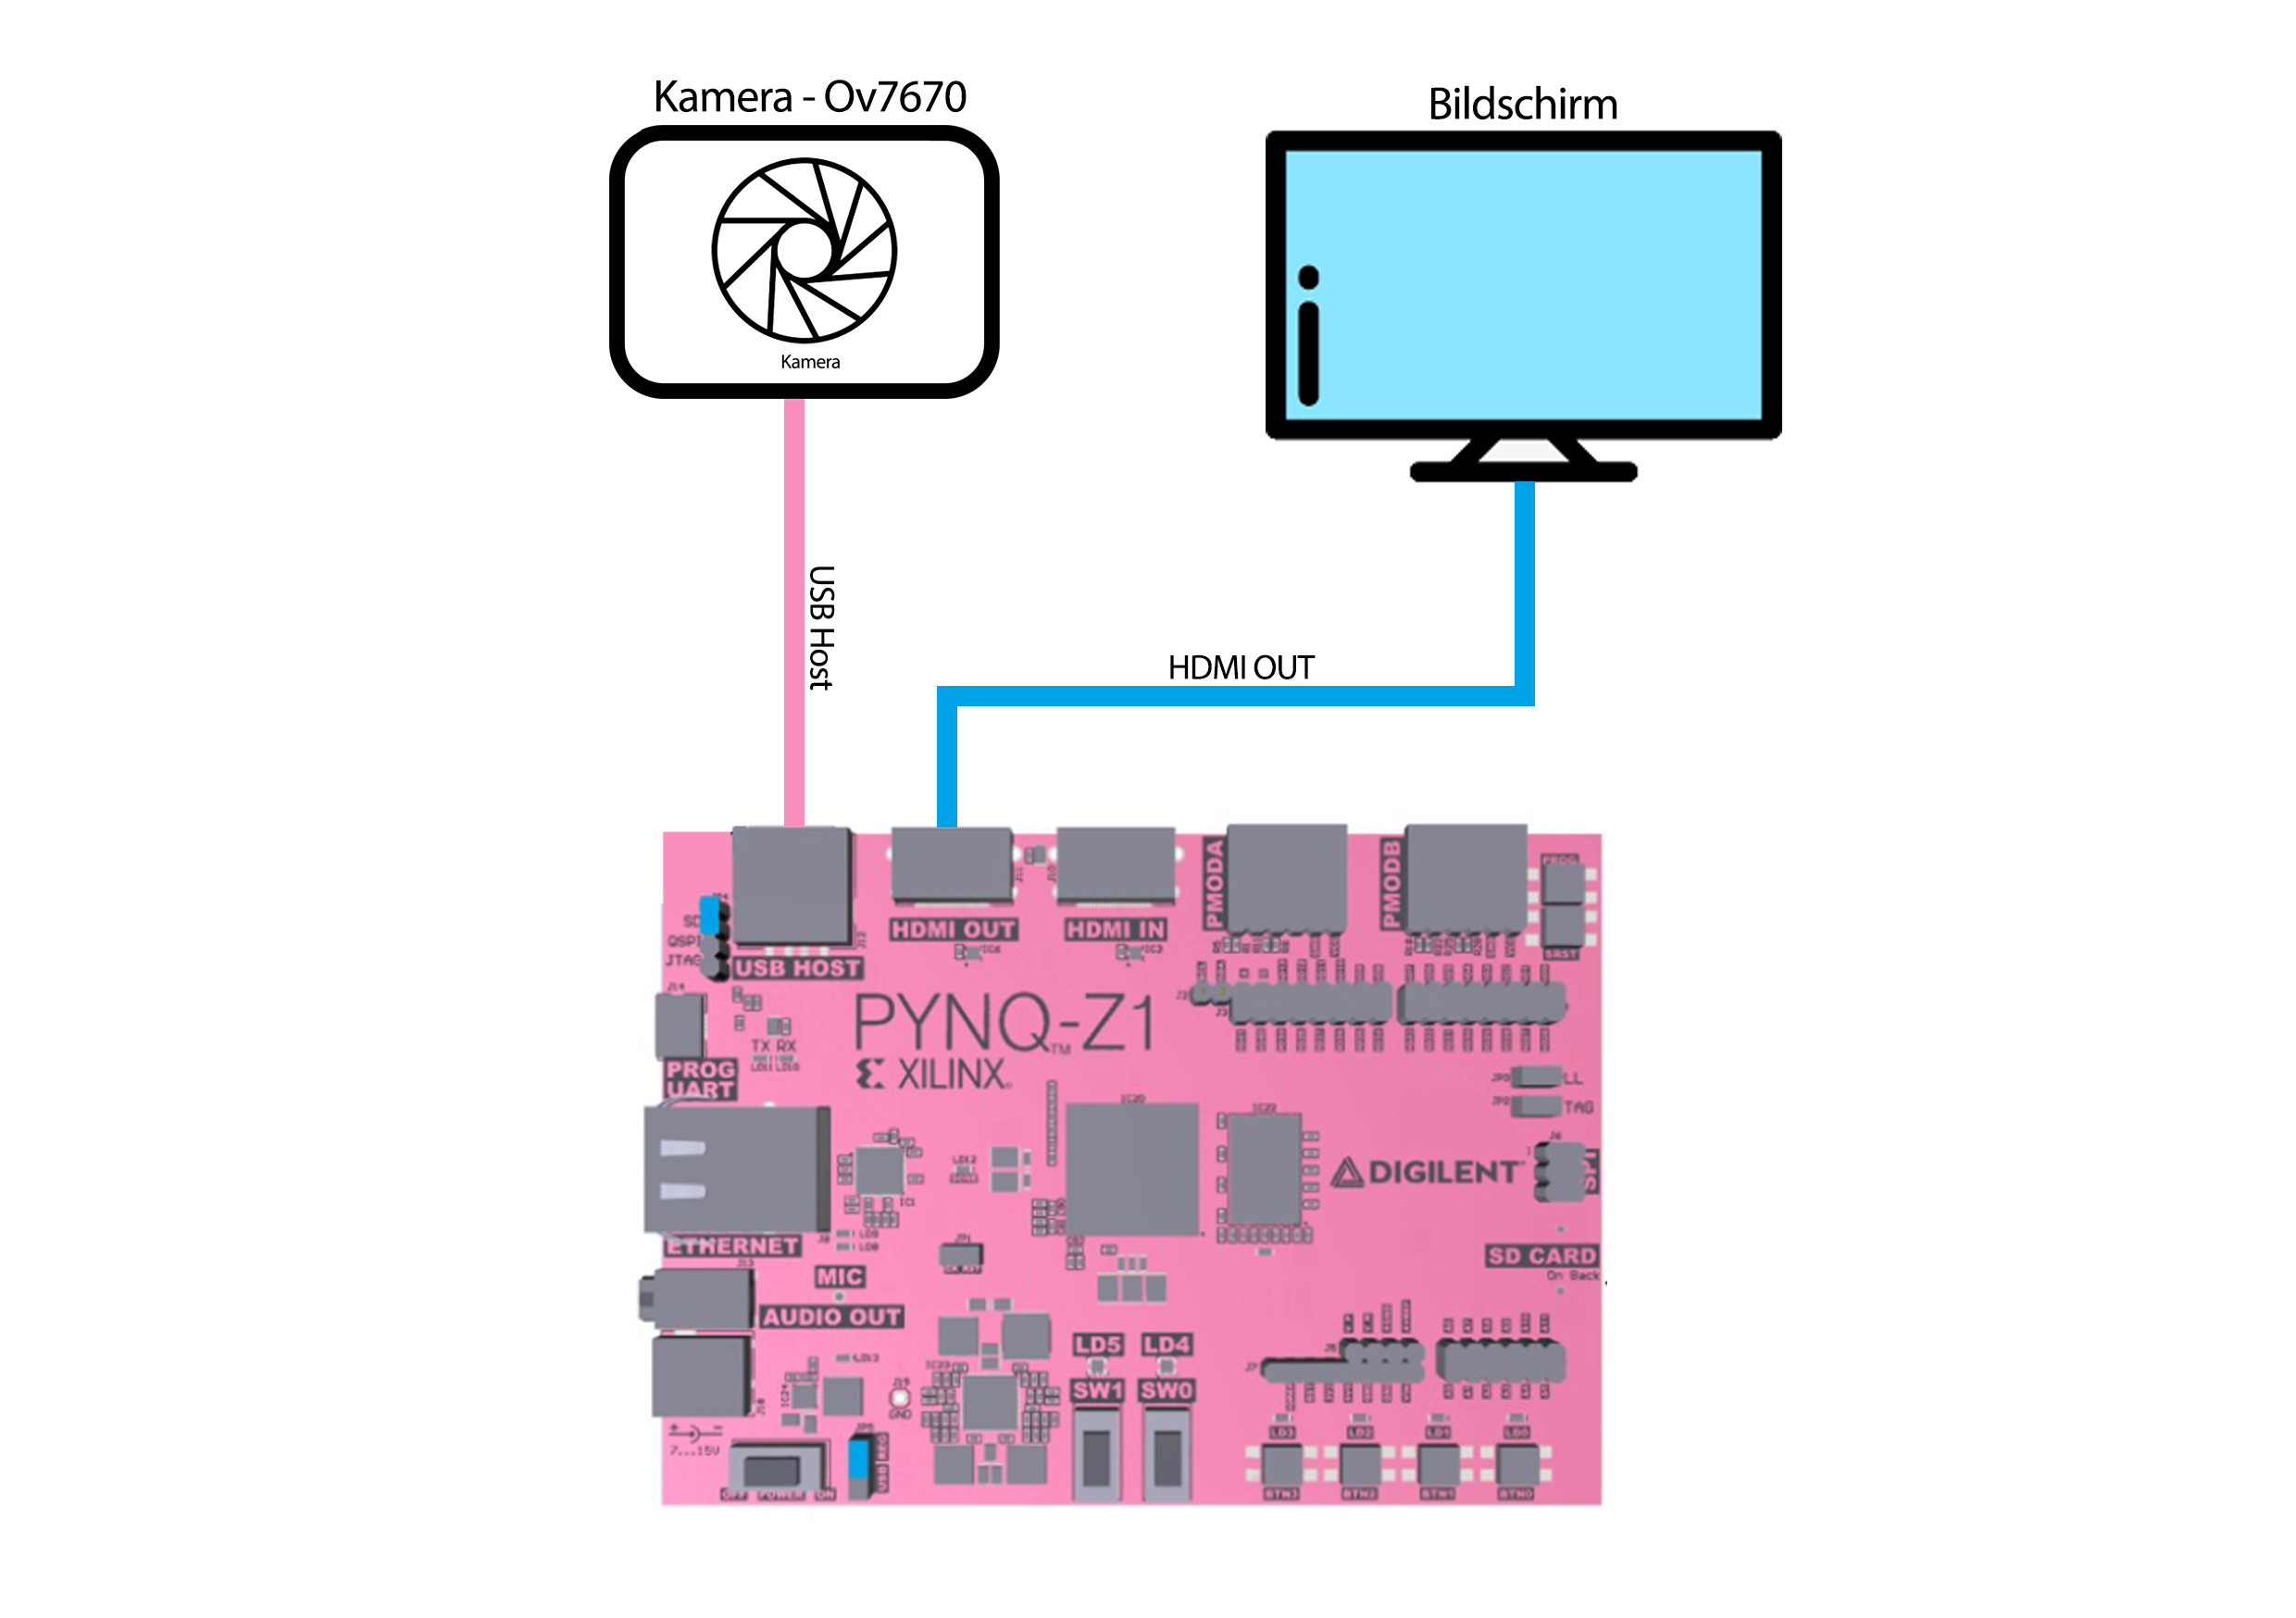
\includegraphics[width=15cm,height=9cm]{PIC/schematikcameraUsb}}
	\caption{Entwurf des Projects durch USB Host und HDMI OUT}
	\label{Entwurf des Projects durch_USB_Host_und_HDMI_OUT}
	\end{figure}

Die zweite Möglichkeit, wie unten im Entwurf gezeigt, wir über die FPGA Pins mit VGA Adapter ein Bildschirm angeschlossen.
	\begin{figure}[H]
	\centering
	\subfloat{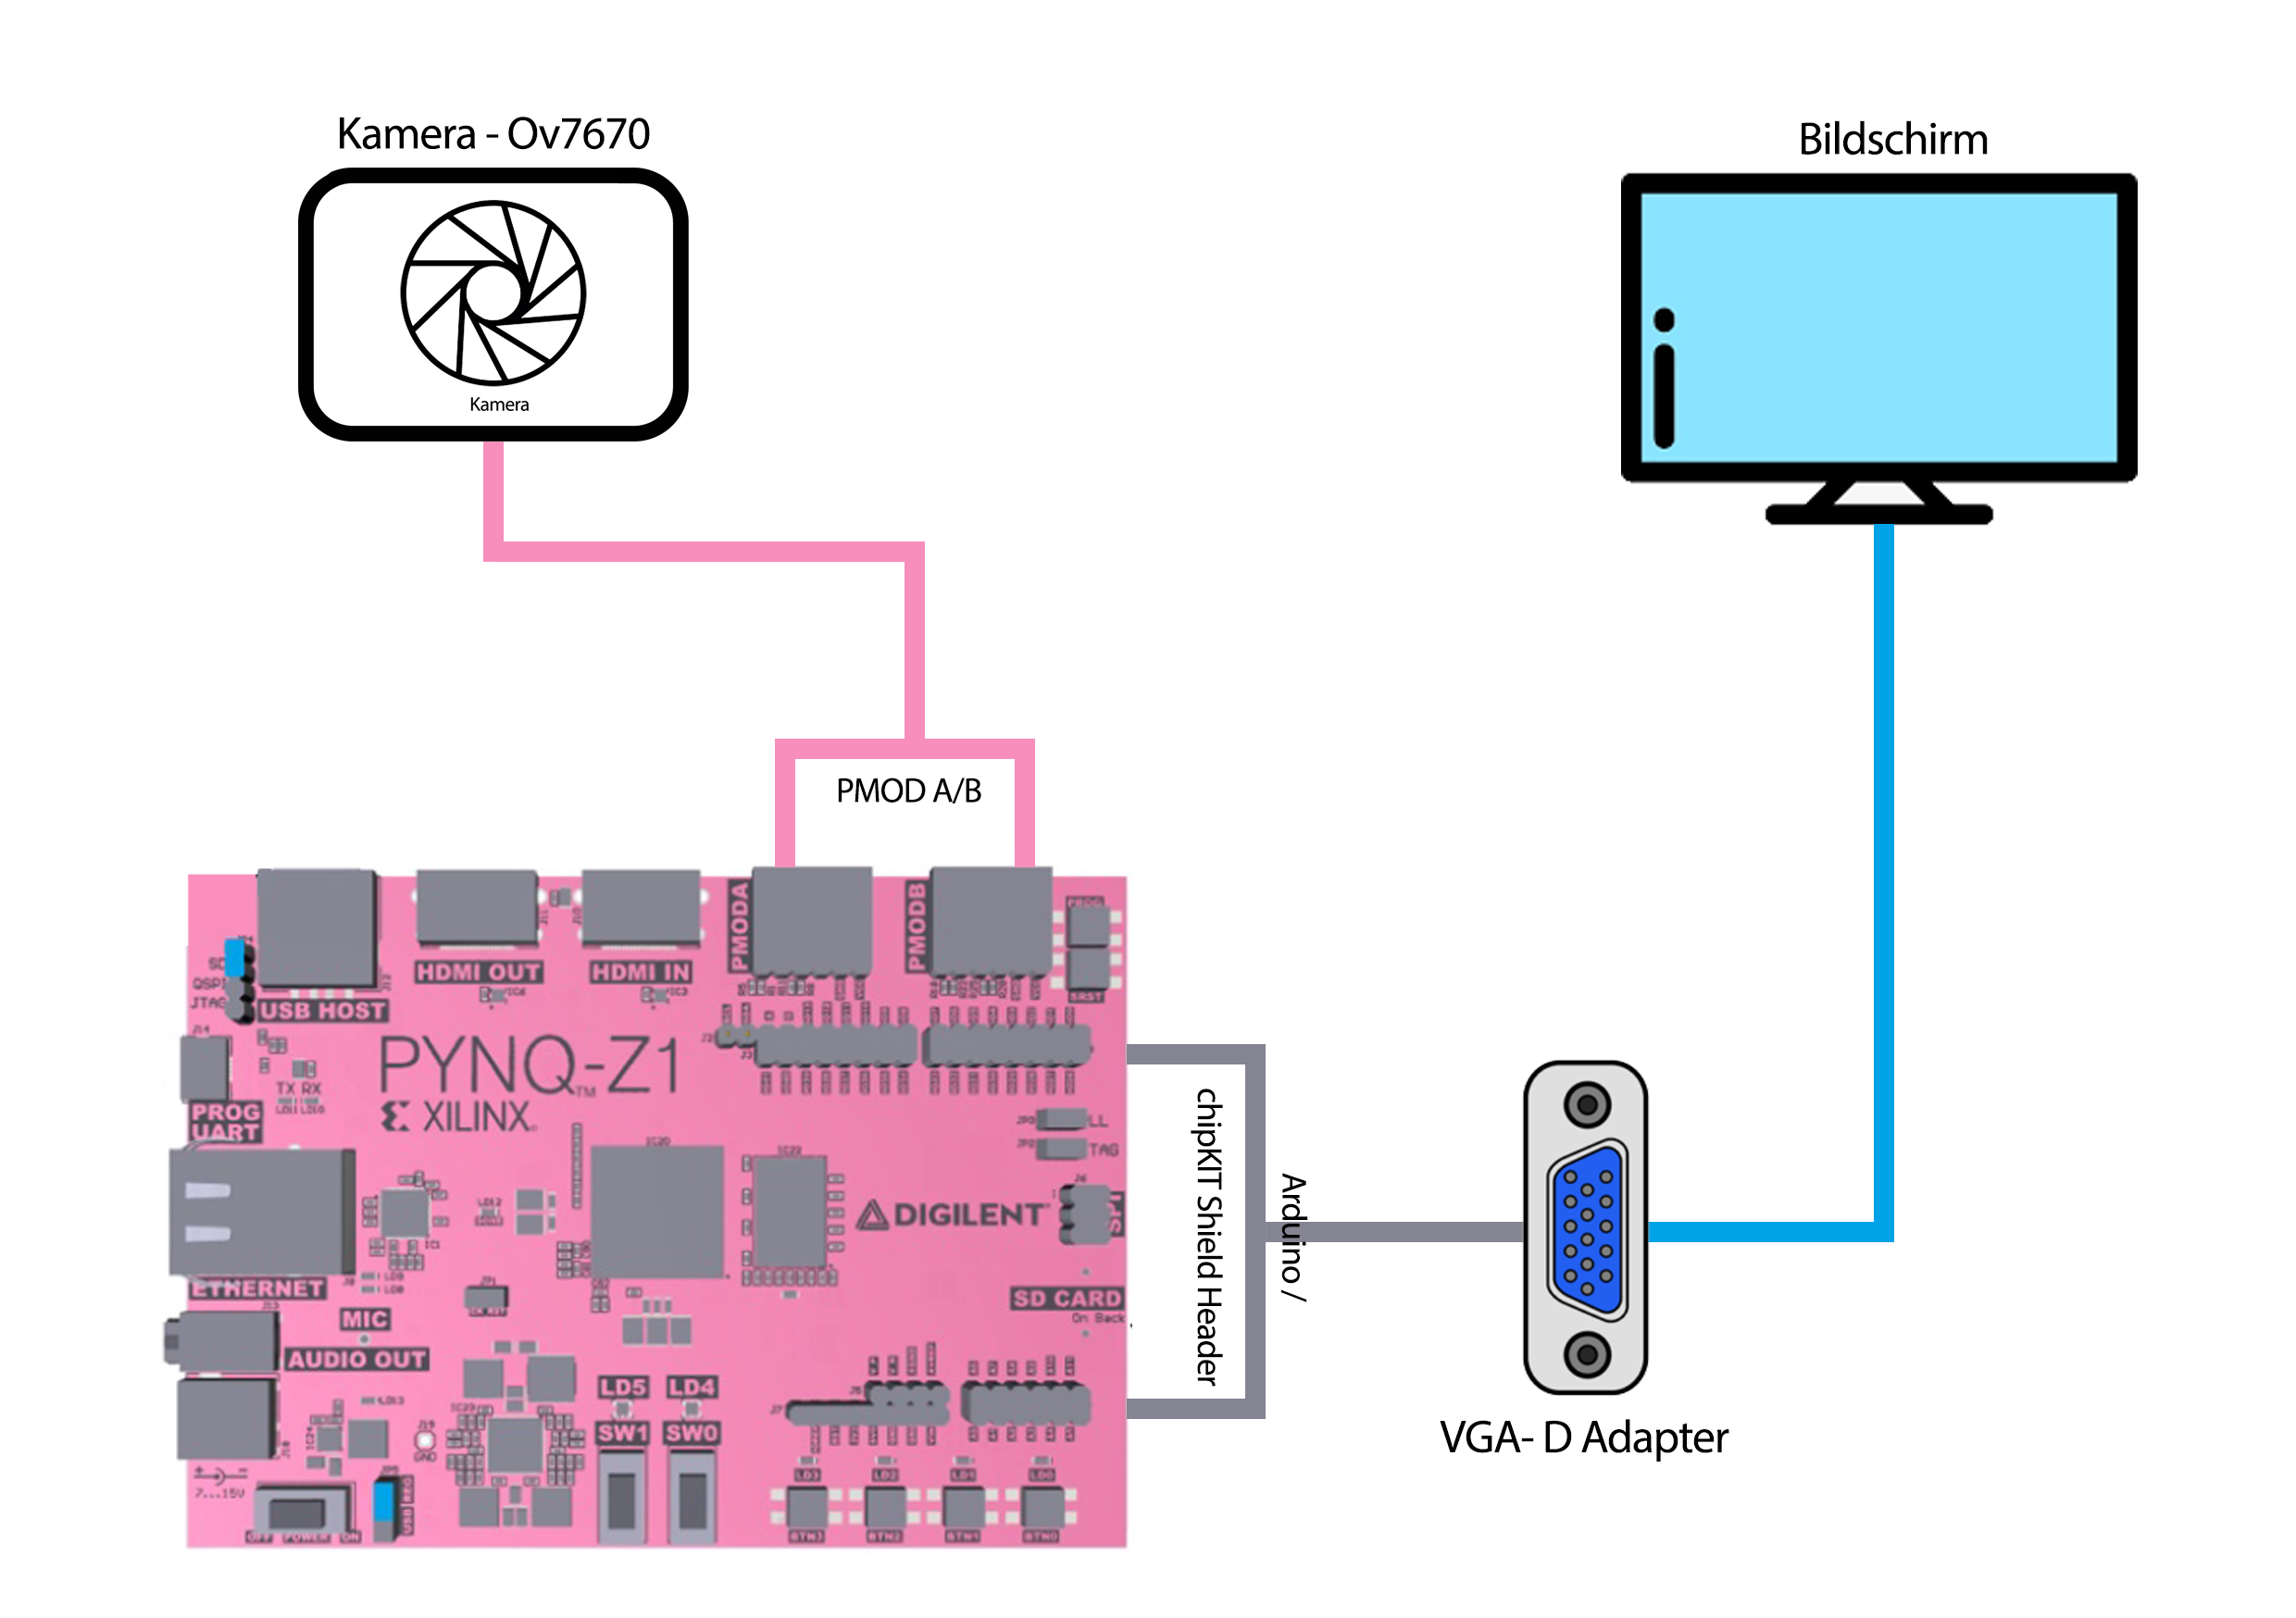
\includegraphics[width=13cm,height=8cm]{PIC/schematik}}
	\caption{Entwurf des Projects durch VGA Adapter}
	\label{Entwurf des Projects durch_VGA_Adapter}
	\end{figure}
	
Die Kamera kann ebenfalls entweder an USB oder PMOD...


\section{Xilinx Pynq-Z1 board}
Das PYNQ-Z1 Board wurde für die Verwendung mit PYNQ entwickelt, einem neuen Open-Source-Framework, das es Embedded-Programmierern ermöglicht, die Fähigkeiten von Xilinx Zynq All Programmable SoCs\footnote{System On Chip} (APSoCs) zu nutzen, ohne programmierbare Logikschaltungen entwickeln zu müssen. Die programmierbaren Logikschaltungen werden als Hardwarebibliotheken importiert und  ihre APIs\footnote{Application Programming Interface} sind im Wesentlichen so programmiert, dass sie wie die Softwarebibliotheken importiert und programmiert werden. Für Designer, die das Basissystem mit neuen Hardware-Bibliotheken erweitern wollen, stehen die Xilinx Vivado WebPACK-Tools kostenlos zur Verfügung.

Das PYNQ-Z1 unterstützt Multimedia-Anwendungen mit integrierten Audio- und Videoschnittstellen und ist so konzipiert, dass es unkompliziert mit Pmod-, Arduino- und Grove-Peripheriegeräten sowie universellen IO-Pins erweiterbar ist.
Ebenso kann das PYNQ-Z1 Board auch mit USB-Peripheriegeräten wie WiFi, Bluetooth und Webcams erweitert werden und ist die Hardware-Plattform für das PYNQ Open-Source-Framework.

	\begin{figure}[H]
	\centering
	\subfloat{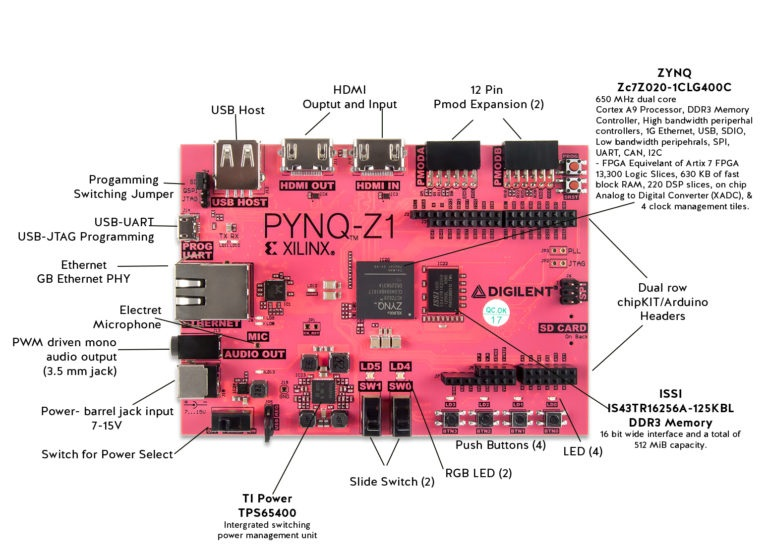
\includegraphics[width=15cm,height=9cm]{PIC/PYNQZ1}}
	\caption{Übersicht PYNQ-Z1}
	\label{Übersicht PYNQ-Z1}
	\end{figure}

Hardwarekomponenten auf dem Pynq-Z1 Board:

	\begin{enumerate} 
	\item 512 MB DDR3 mit 16-bit Bus bei 1050Mbps.
	\item 650 MHz Dual-Core Cortex-A9 Prozessor.
	\item 16 MB Quad-SPI\footnote{Serial Peripheral Interface} Flash, werkseitig programmiertem.
	\item Peripherie-Controller mit niedriger Bandbreite: SPI, UART, KANN, I2C.
	\item 630 KB fast block RAM.
	\item13,300 Logikscheiben mit je vier 6 Eingangs-LUT und 8 Flip-Flops.
	\item u.s.w\\
	\end{enumerate}

\subsection{PYNQ Z1 Core}
Das PYNQ-Z1 besteht aus einem Zynq-XC7Z020-1CLG400C (xc7z020dg400-1) SoC, der wiederum einen dual Core ARM Cortex-A9 und einen Artix-7 FPGA enthält:

	\begin{figure}[H]
	\centering
	\subfloat{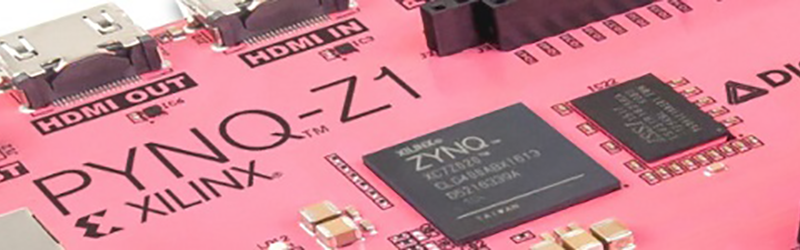
\includegraphics[width=8cm]{PIC/pynqcore}}
	\caption{PYNQ Z1 Core}
	\label{PYNQ Z1 Core}
	\end{figure}


\subsection{Power Jumper}

PYNQ Z1 hat 2 \textbf{''Modi''} Formen der Spannungsversorgung. Die Modi werden durch die Änderung des Power Jumpers JP5 gewählt.

\begin{enumerate} 
\item \textbf{USB} über Anschluss J14 (PROG oder UART)
\item  \textbf{REG} über Anschluss J18 (External Power)\\
\end{enumerate}

\textbf{Hinweis1 :} Die Ausgangsspannung \textbf{AC} muss zwischen 7VDC und 15VDC sein.
	
\textbf{Hinweis2 :} Wenn die Eingangsspannungen \textbf{>15VDC} sein, wird das Board beschädigt.



	\begin{figure}[H]
	\centering
	\subfloat{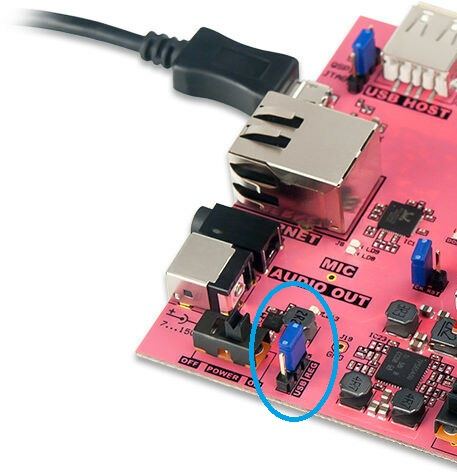
\includegraphics[width=5cm]{PIC/Jumper_Netzteil}}
	\caption{Power Jumper JP5}
	\label{Power_Jumper}
	\end{figure}



\subsection{Programming Switching Jumper (Boot Jumper)}

Der Bootmodus wird mittels Jumper JP4 gewählt. Das Board kann über SD-Karte, Quad SPI oder JTAG gebootet werden.

	\begin{figure}[H]
	\centering
	\subfloat{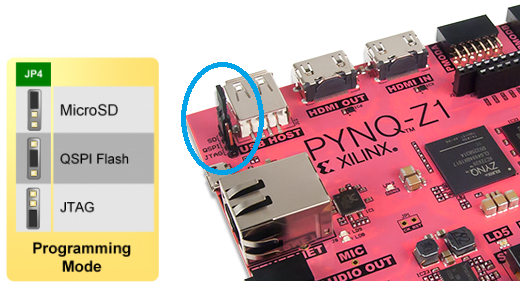
\includegraphics[width=5cm]{PIC/BootJumper}}
	\caption{Boot Jumper JP4}
	\label{Boot_Jumperr}
	\end{figure}

Die drei Startmodi werden im folgenden Text beschrieben: 

	\begin{enumerate} 
	\item   \textit{microSD Boot Mode}
	
	Der PYNQ-Z1 unterstützt \textbf{Booting} von einer microSD-Karte, die in Anschluss \textbf{J9} eingesetzt ist.
	
	\item  \textit{Quad SPI Boot Mode}
	
	Der PYNQ-Z1 verfügt über einen integrierten 16-MB-Quad-SPI-Flash, von dem der Zynq booten kann.
	
	\item  \textit{JTAG Boot Mode}
	
	Wenn der Prozessor in den JTAG-Startmodus versetzt wird, wartet er, bis die Software mithilfe der Xilinx-Tools von einem Host-Computer geladen wird.\\
Nach dem Laden der Software kann die Software entweder mit der Ausführung beginnen oder mit dem Xilinx SDK zeilenweise durchlaufen werden.
	\end{enumerate}

\subsection{microSD Slot}

Der PYNQ-Z1 bietet einen microSD-Slot\footnote{Steckplatz} (J9) für \textit{''non-volatile''} externen Speicher sowie zum Booten des Zynq.
Der Steckplatz ist mit Bank 1/501 MIO [40-47] auch einschließlich Card Detect verbunden.

	\begin{figure}[H]
	\centering
	\subfloat{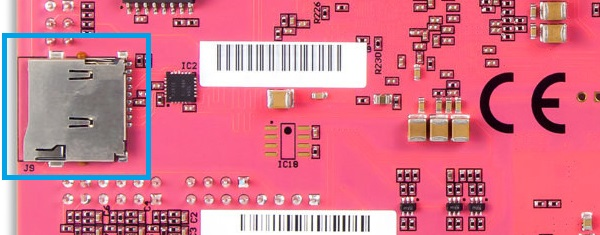
\includegraphics[width=7cm]{PIC/SDcard}}
	\caption{microSD-Slot}
	\label{microSD_Slot}
	\end{figure}
	
	
\textbf{Hinweis:} Für das Betriebssystem wird mindestens eine\textbf{ Klasse-4 Karte} mit \textbf{8 GB Speicherplatz} empfohlen.

Informationen zum Einrichten und Verwendung der Speicherkarte finden Sie im Abschnitt Software und im Bereich \textbf{\nameref{Einrichtung_der_Speicherkarte}}.



\subsection{HDMI IN/OUT}

Die PYNQ-Z1-Karte enthält einen HDMI-Eingangsanschluss und einen HDMI-Ausgangsanschluss, die mit dem FPGA-Fabric des Zynq Chips verbunden sind.
Dies bedeutet, dass zur Verwendung der HDMI-Anschlüsse die HDMI-Controller in einer Hardware-Bibliothek oder einem Overlay enthalten müssen.

	\begin{figure}[H]
	\centering
	\subfloat{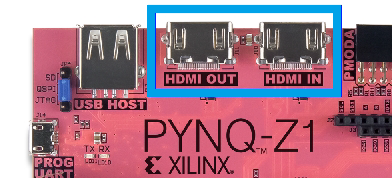
\includegraphics[width=7cm]{PIC/HDMIINOUT}}
	\caption{HDMI IN/OUT}
	\label{HDMI_IN_/_OUT}
	\end{figure}

Das Basis-Overlay enthält einen HDMI-Eingangscontroller und einen HDMI-Ausgangscontroller, die beide an die entsprechenden HDMI-Anschlüsse angeschlossen sind.\\
Am Zynq PS ist ein USB-Controller angeschlossen. Eine Webcam kann auch zum Aufnehmen von Bildern oder Videoeingaben verwendet werden, die über den HDMI-Ausgang verarbeitet und angezeigt werden können.


\subsection{USB-HOST}
Der PYNQ-Z1 implementiert eine der beiden verfügbaren PS-USB-OTG\footnote{On-The-Go}-Schnittstellen auf dem Zynq-Gerät.
Als PHY wird ein Microchip USB3320 USB 2.0 Transceiver-Chip mit einer 8-Bit-ULPI-Schnittstelle verwendet.

	\begin{figure}[H]
	\centering
	\subfloat{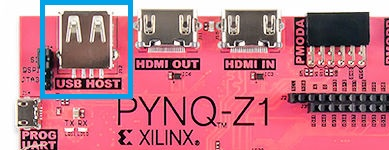
\includegraphics[width=7cm]{PIC/USBHOST}}
	\caption{USB Host}
	\label{USB_Host}
	\end{figure}

Das PHY verfügt über ein komplettes HSUSB Physical Front-End, das Geschwindigkeiten mehr als 480 MBit / s unterstützt.\\
Der PHY ist an die MIO Bank 1/501 angeschlossen, die mit 1,8 V versorgt wird. Das USB0-Peripheriegerät wird an der PS verwendet, die über MIO [28-39] angeschlossen ist.\\
\textbf{Hinweis:} USB OTG ist eine Variante des Universal Serial Bus (USB), die es einem USB-Gerät ermöglicht, eingeschränkte USB-Host-Aufgaben zu übernehmen.


\subsection{PMOD A/B}
\label{PMODE_PORTS}

Ein Pmod-Port ist eine offene 12-polige Schnittstelle, die von einer Reihe von Pmod-Peripheriegeräten unterstützt wird.\\

Typische Pmod-Peripheriegeräte sind:
	
	\begin{itemize}
		\item Sensoren (Spannung, Licht, Temperatur)
		\item Kamera
		\item Kommunikationsschnittstellen (Ethernet, seriell, WLAN, Bluetooth) 
		\item Eingangs- und Ausgangsschnittstellen (Tasten, Schalter, LEDs)
	\end{itemize}

		\begin{figure}[H]
			\centering
			\subfloat{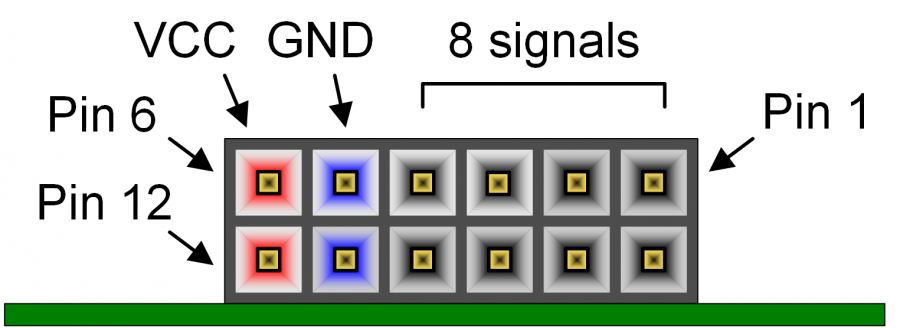
\includegraphics[width=7cm]{PIC/pynqPmod}}
			\qquad
			\subfloat{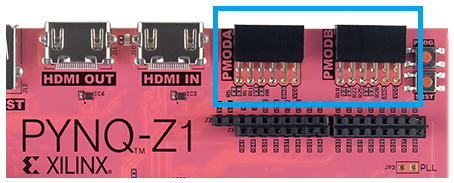
\includegraphics[width=7cm]{PIC/pmodport}}
			\caption{PYNQ PMODE Pins und PYNQ PMODE Ports }
			\label{fig:PYNQ_PMODE_PYNQ_PMODE_Ports}
		\end{figure}


	
High-Speed Pmod ports, jeder 12 Pins Pmod-Port liefert zwei 3,3 VCC Signale (Pins 6 und 12), zwei Groundssignale (Pins 5 und 11) und 8 Logiksignale.\\

\textbf{Hinweis:} Da die Pins nicht gegen Kurzschluss oder Überspannung (>3.3V) geschützt sind, muss beim Verdrahten
besonders aufgepasst werden.\\\\
Aufgrund der Verwendung dieser Komponente  im Projekt werden wird in den folgenden Kapiteln und der \textbf{\nameref{Implementierung_des_Projeks}}-Abschnitt vollständig erklärt.


\subsection{Arduino / chipKIT Shield Header}
Der PYNQ-Z1 kann an Standard-Arduino und ChipKIT Shields angeschlossen werden, um die Funktionalität zu erweitern.
Der Shield Connector verfügt über 49 Pins, die für allgemeine digitale E / A mit dem Zynq PL verbunden sind.

	\begin{figure}[H]
	\centering
	\subfloat{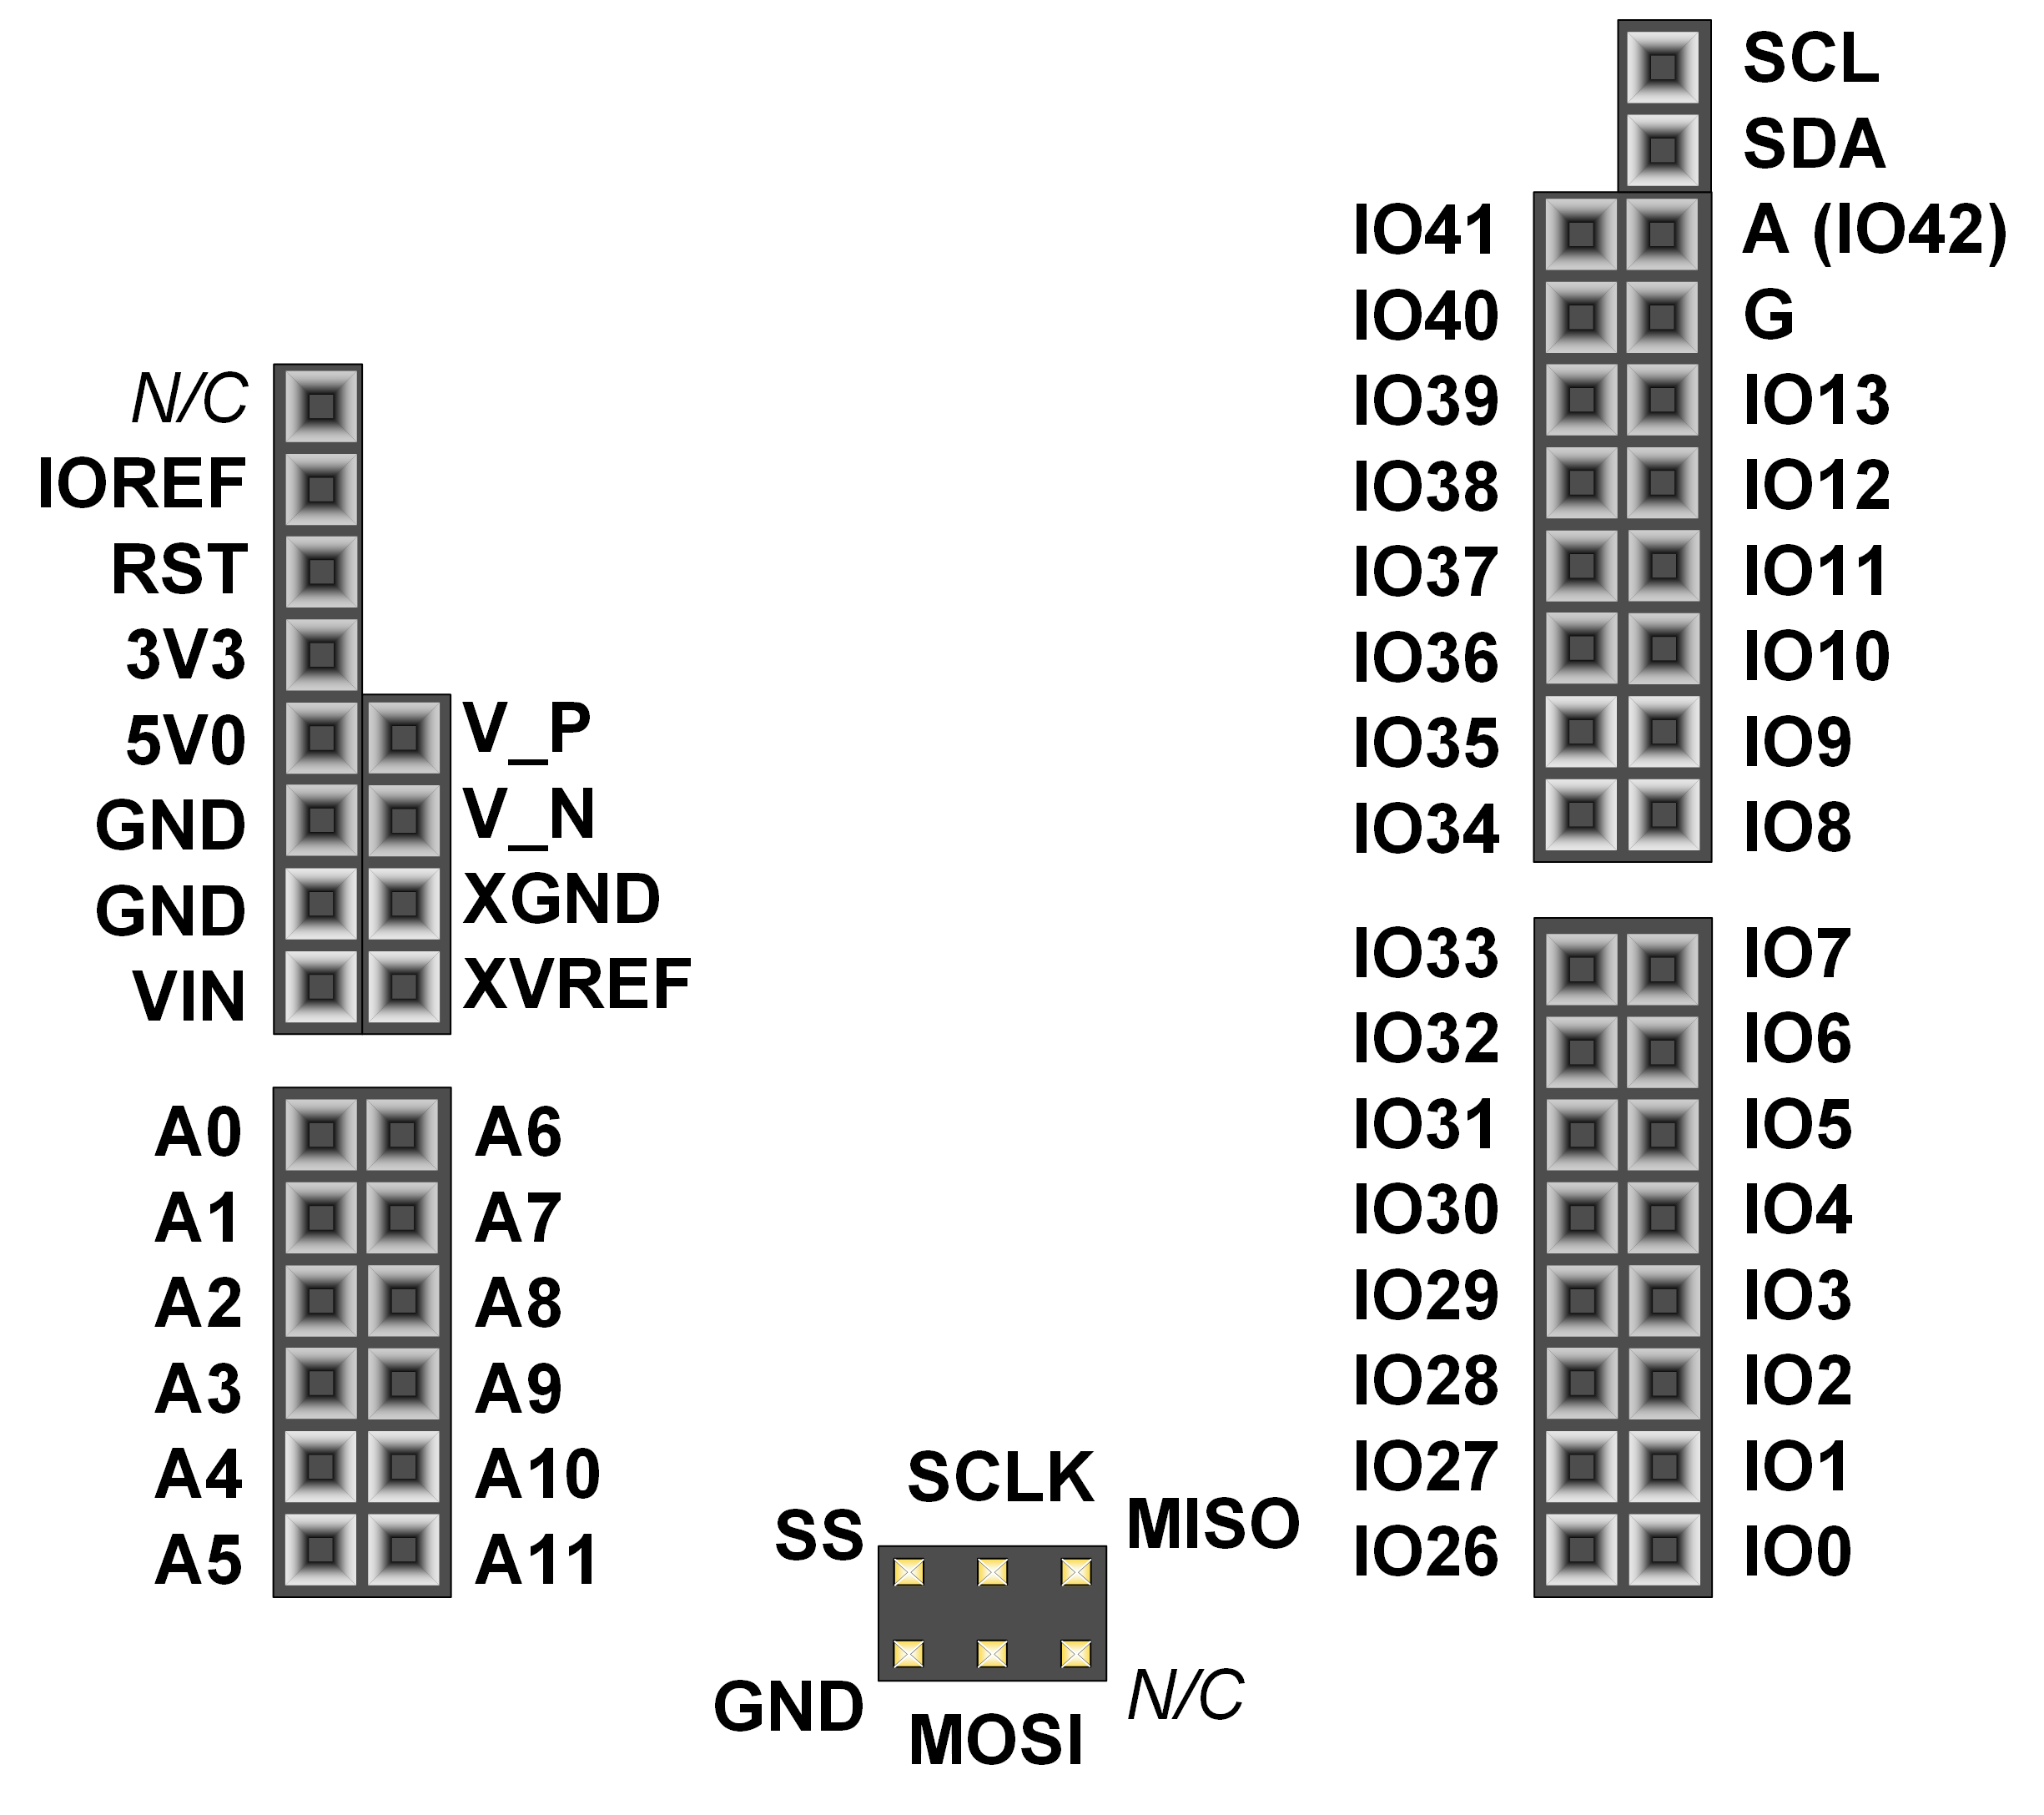
\includegraphics[width=7cm]{PIC/pynqz1shield}}
	\caption{Shield Pin Diagram}
	\label{fig:Shield_Pin_Diagram}
	\end{figure}

Aufgrund der Flexibilität von FPGAs können diese Pins für nahezu alles verwendet werden, einschließlich digitalem Lesen / Schreiben, SPI-Verbindungen, UART-Verbindungen, I2C\footnote{I-squared-C protocol}Verbindungen, VGA Controller und PWM.

6 dieser Pins (mit AN0-AN5 bezeichnet) können auch als unsymmetrische Analogeingänge mit einem Eingangsbereich von 0 V bis 3,3 V verwendet werden, und weitere 6 (mit AN6-11 bezeichnet) können als differentielle Analogeingänge verwendet werden.\\

	\textbf{Hinweis1 :} Der PYNQ-Z1 ist \textbf{nicht} mit Shield kompatibel, die 5-V-Digital- oder Analogsignale ausgeben.
	
	\textbf{Hinweis2 :}  Mehr als \textbf{5 V} kann die Driving pins am PYNQ-Z1- Shield Connector beschädigen.



\subsection{Ethernet}
Der PYNQ-Z1 verwendet einen Realtek RTL8211E-VL PHY, um einen 10/100/1000 Ethernet-Port für die Netzwerkverbindung zu implementieren.

	\begin{figure}[H]
	\centering
	\subfloat{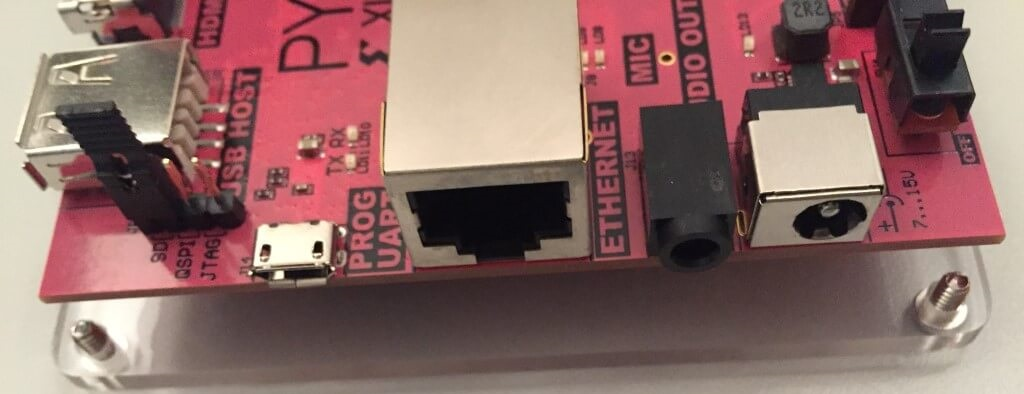
\includegraphics[width=7cm]{PIC/PYNQZ1Ethernet}}
	\caption{Ethernet}
	\label{fig:Ethernet}
	\end{figure}

Das Board versucht nach dem Anschalten über DHCP eine IP-Adresse zu erhalten und fällt auf \sout{192.168.3.99/24} 192.168.3.99:9090 zurück, falls kein DHCP Server verfügbar ist.\\

\textbf{Hinweis:} IP-Adressen Port hängt von der Version des Image Files \textbf{pynq{\_}z1{\_}v2.1.img}, z.B. bei Version 2.0 lautet 192.168.2.99:9090 und es ist möglich, dass bei einer anderen Version als 2.0 die Ip-Adresse angepasst werden muss.\\
	
Der PYNQ-Z1 enthält auch andere Komponenten wie MIC/AUDIO OUT, Schalter, Taster, RGB LEDs, u.s.w.\\\\
Weitere Informationen zu diesen Teilen finden Sie im PYNQ-Z1-Handbuch.




\section{Kamera - Ov7670}
Der OV7670 verwendet den RGB565-Modus mit 30 Bildern pro Sekunde. Die Frames können im internen BRAM\footnote{BLOCK RAM} des 7Z020 des ZYNQ7-Chips gespeichert werden. Der VGA-Controller liest die Daten aus dem Block Ram und verwendet eine 12-Bit-Farbtiefe auf dem VGA-Schnittstellenbildschirm.\\
Die VGA-Auflösung beträgt ebenfalls 640x480. Die Kamera wird mit +3,3V versorgt.

		\begin{figure}[H]
			\centering
			\subfloat{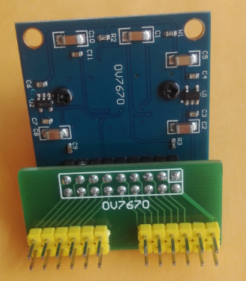
\includegraphics[width=4cm]{PIC/Ov7670camera_Back}}
			\qquad
			\subfloat{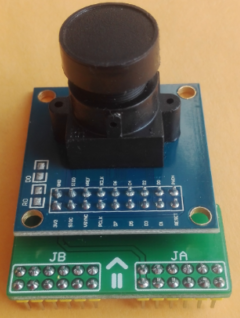
\includegraphics[width=3.45cm]{PIC/Ov7670camera_Front}}
			\caption{Kamera - Ov7670}
			\label{fig:Kamera - Ov7670}
		\end{figure}


\textbf{Hinweis: } 7Z020 verfügt über einen umfangreichen BLOCK RAM-Block, sodass Sie 640X480 = 307200 12-Bit-Nummern direkt speichern können, sodass kein externer Speicher für die Videopufferung verwendet wird.

Bemerkenswerte Eigenschaften dieser Kamera sind:
	\begin{itemize}
		\item Steuerung den SCB\footnote{Storz Communication Bus}-Busteil
		\item Broad stopband performance bis to 8 GHz
		\item Fast roll-off
		\item Connectorized package
	\end{itemize}



\section{VGA- D Adapter}
Es ist Kleine Platine mit 16 poligem Terminalblock ( Klemmleisten 3,81mm Raster) auf eine 3-reihige High Density Buchse für VGA\footnote{Video Graphics Array} Anwendungen.
VGA- D Adapter umfasst die Spezifikation einer analogen elektronischen Schnittstelle zur Übertragung von Bildern oder Videos zwischen unseren Board und Bildschirm sowie Spezifikationen für hierzu geeignete Stecker und Kabel.


		\begin{figure}[H]
			\centering
			\subfloat{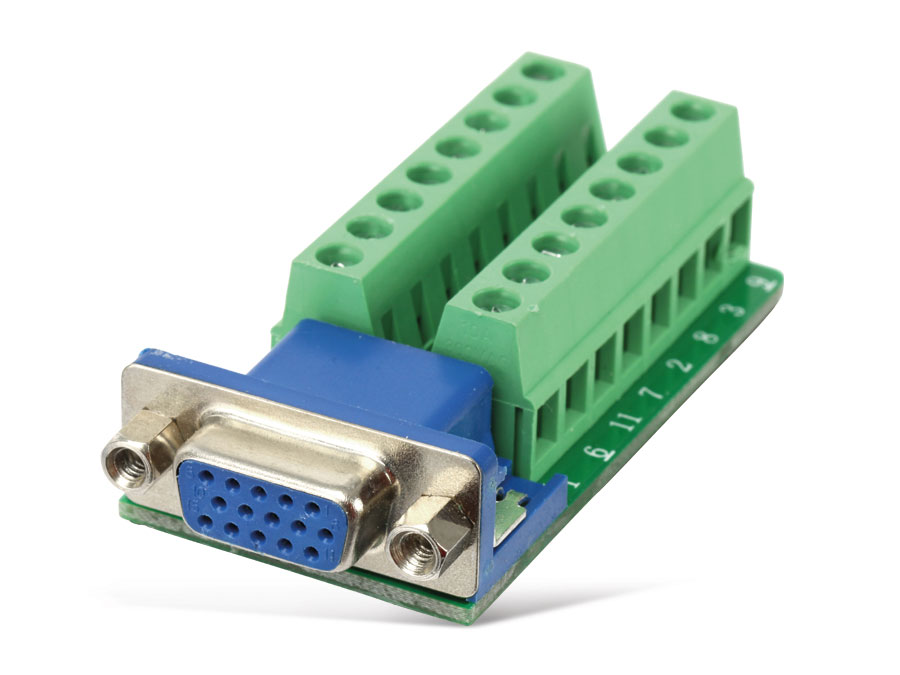
\includegraphics[width=5cm]{PIC/AdapterVGA2}}
			\qquad
			\subfloat{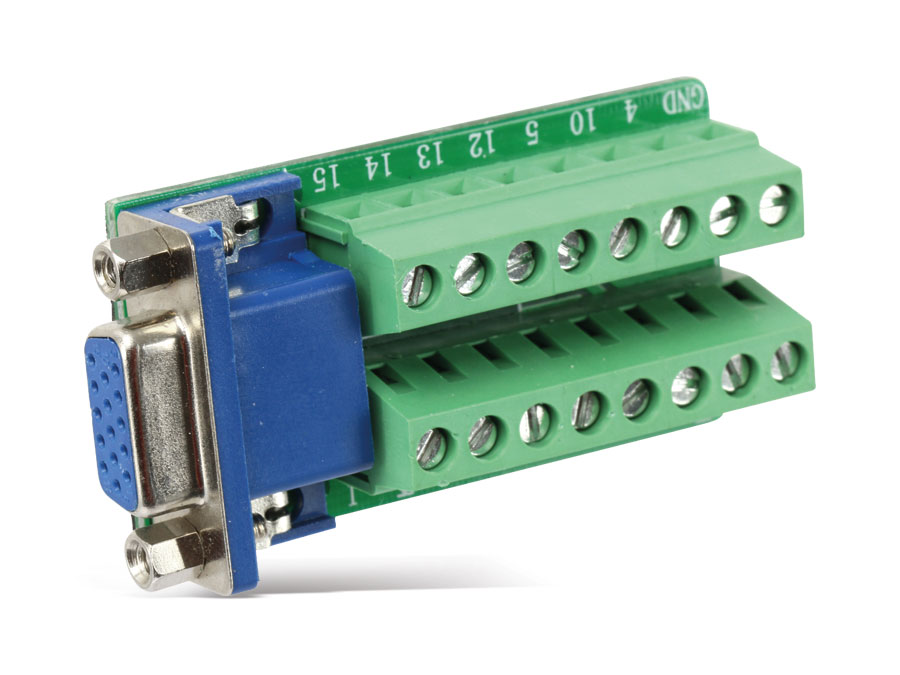
\includegraphics[width=5cm]{PIC/AdapterVGA1}}
			\caption{VGA D Adapter}
			\label{fig:VGA_Adapter}
		\end{figure}




	%------------------------------------------------
	%	3. Chapter
	%------------------------------------------------

\chapter{Softdware}

	
\section{Einrichtung der SDkarte}
\label{Einrichtung_der_SDkarte}


Mit dem folgenden Verfahren können Sie den Zynq von microSD mit einem Standard-\textbf{Zynq-Boot-Image} starten, das mit den Xilinx-Tools erstellt wurde:

	\begin{enumerate} 
	
		\item Formatieren Sie die microSD-Karte mit einem FAT32-Dateisystem.
		\item Kopieren Sie das mit Xilinx SDK erstellte \textbf{Zynq Boot Image} auf die microSD-Karte.
		\item Benennen Sie das Zynq-Boot-Image auf der microSD-Karte in\textbf{ BOOT.bin }um.
		\item Entnehmen Sie die microSD-Karte aus Ihrem Computer und stecken Sie sie in den Anschluss\textbf{ J9} des PYNQ-Z1.
		\item Schließen Sie eine\textbf{ Stromquelle} an den PYNQ-Z1 an und wählen Sie sie mit\textbf{ JP5 }aus.
		\item Stecken Sie einen einzelnen\textbf{ Jumper} auf \textbf{ JP4 } und schließen Sie die beiden oberen Stifte (mit der Bezeichnung „SD“) kurz.
		\item Schalten Sie die Karte ein. Das Board bootet nun das Image von der microSD-Karte.

	\end{enumerate}

	%------------------------------------------------
	%	4. Chapter
	%------------------------------------------------

\chapter{Implementierung des Projeks}
\label{Implementierung_des_Projeks}


\section{Hardwares Implementierung}

\subsection{Einstellung von Pmod port}
Wie im Abschnitt \textbf{\nameref{PMODE_PORTS}} schon erwähnt wurde, 


\section{HLS Software Implementierung}










	%------------------------------------------------
	%	Literaturverzeichnis
	%------------------------------------------------


\begin{thebibliography}{9}

\bibitem{PYNQ-Z1 Board} 
Xilinx PYNQ Z1 Board,
\\\texttt{https://blog.digilentinc.com/python-zynq-pynq-introducing-our-latest-collaborationl}

\bibitem{PYNQ-Z1} 
PYNQ Z1-Komponenten,
\\\texttt{https://buildmedia.readthedocs.org/media/pdf/pynq/v1.4/pynq.pdf}

\bibitem{PYNQ-Z1}
PYNQ Z1-Einrichtung,
\\\texttt{Pynq{\_}Labor{\_}Doku{\_}Jaschko{\_}Stolle.pdf}

\bibitem{Ov7670camera} 
Ov7670camera,
\\\texttt{http://www.alselectro.com/arduino-camera-ov7670.html}

\end{thebibliography}




\end{document}